\documentclass[aspectratio=169]{beamer}
\setbeamertemplate{navigation symbols}{} % don't use navigation tools on slides
% \usetheme{LMT}

\usepackage[utf8]{inputenc}
\usepackage{pdfpc-commands}
\usepackage{multimedia}
\usepackage{listings}
\usepackage{default}
\usepackage{xcolor}

\setbeamersize{text margin left=0.6cm,text margin right=0.6cm}
\setbeamercolor{frametitle}{fg=black}
\setbeamercolor{section in toc}{fg=black}
\setbeamertemplate{frametitle}{\color{black}\bfseries\insertframetitle\par\vskip-6pt{\color{gray}\hrulefill}}

\lstset{language=C++,
  basicstyle=\ttfamily,
  keywordstyle=\color{blue}\ttfamily,
  stringstyle=\color{red}\ttfamily,
  commentstyle=\color{green}\ttfamily,
  morecomment=[l][\color{magenta}]{\#}
}

\AtBeginSection[]{
  \begin{frame}{Summary}
    \tableofcontents[currentsection]
  \end{frame} 
}

\begin{document}

\begin{frame}
    \begin{center}
        {\huge High Performance Computing of Power Diagrams}

        \bigskip
        {\large Applications to Semi-Discrete Optimal Transport}
      
        \vfill
        {(MAGA days, November 21, 2019, Hugo Leclerc)}
    \end{center}
\end{frame}

% ---------------------------------------------------------------------------------------
\section*{Introduction}

\begin{frame}
    \frametitle{The world needs power diagrams !}

    \begin{minipage}[c][0.6\textheight][c]{0.5\textwidth}
        Optimal way to transport a density to a set of diracs (equal mass) ? 
        
        \vfill
        Quadratic cost (euclidian distance) $\Rightarrow$ \textit{attributions} are defined by power diagrams.
        
        \vfill
        $x$ is in cell $i$ if $\forall j \neq i$,
         $$|| x - \rho_i ||^2 - \omega_i < || x - \rho_j ||^2 - \omega_j $$
    \end{minipage}
    \kern 0.5cm
    \begin{minipage}{0.45\textwidth}
        \begin{center}
            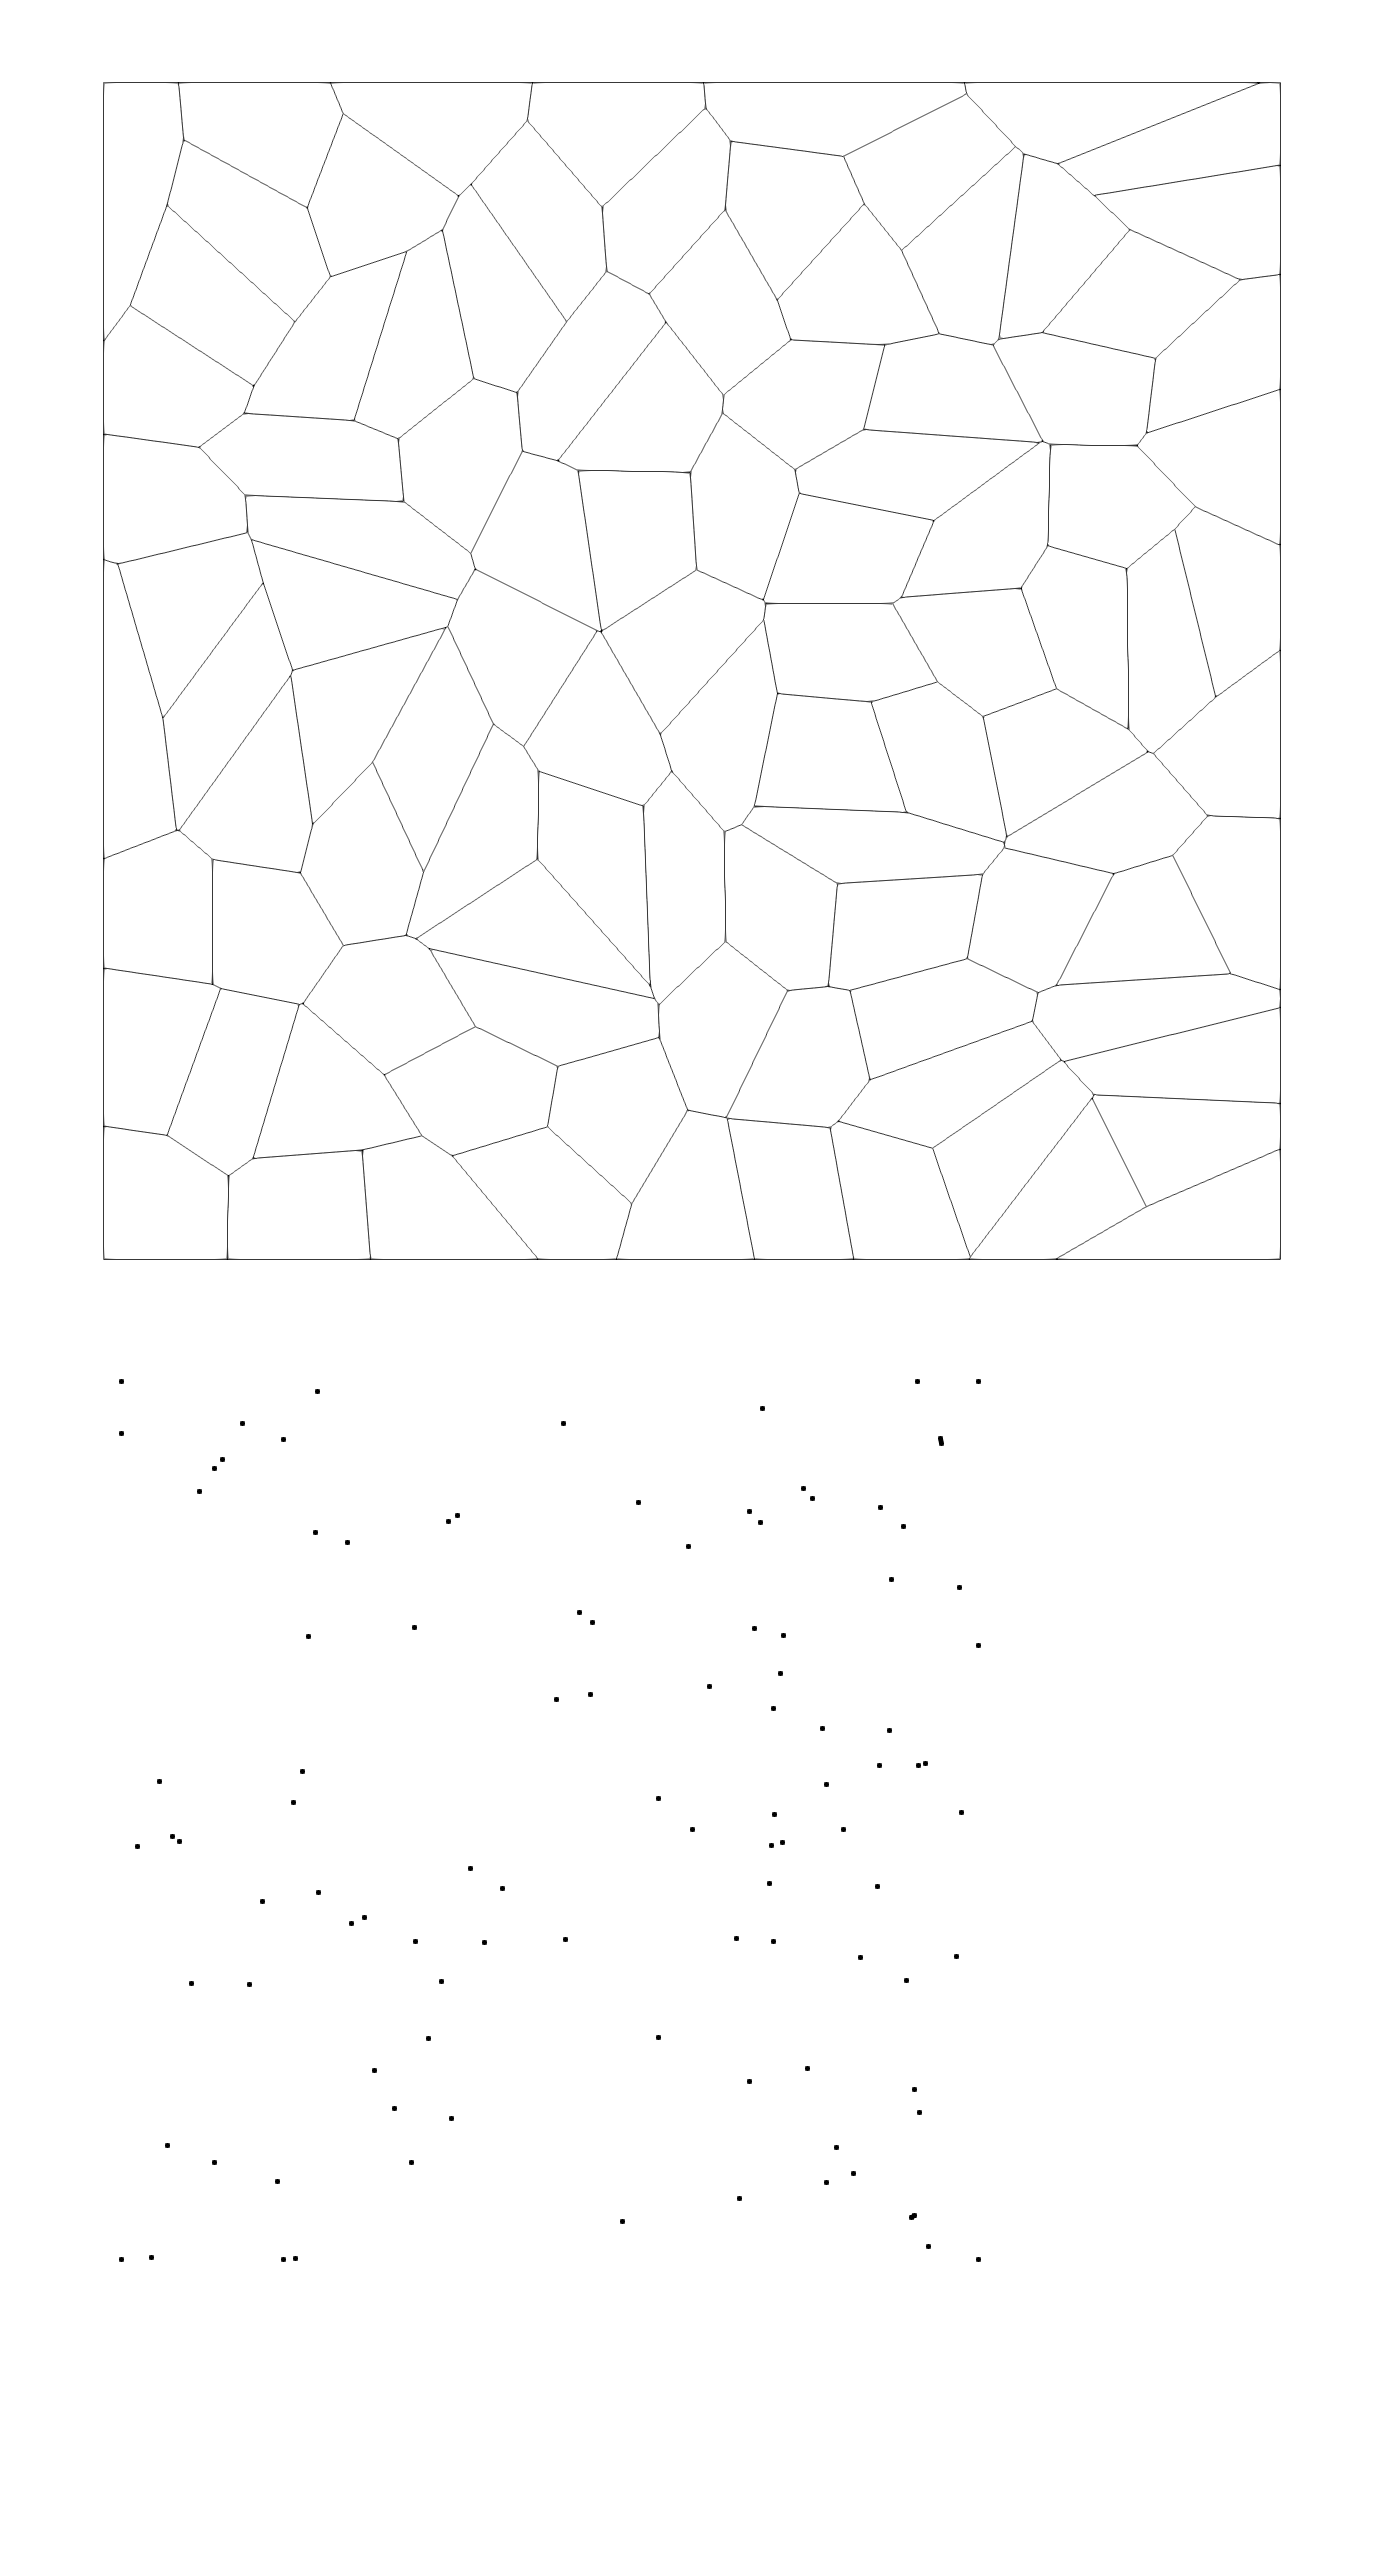
\includegraphics[height=0.8\textheight]{img/pd.png}
        \end{center}
    \end{minipage}
\end{frame}

\begin{frame}
    \frametitle{The world needs efficient power diagram computations !}

    Lot of work done before (Geogram, CGAL, ...), with a focus on the generic case.
    
    \vfill
    Most of the libraries are designed to give an \textit{exact connectivity}
    \begin{itemize}
        \item extra CPU and memory cost (bookkeeping)
        \item essentially sequential
    \end{itemize}

    \vfill
    SDOT application being more relaxed (need for simple integrals)
    \begin{itemize}
        \item development and test opportunities 
        \item scalability
    \end{itemize}
\end{frame}

\begin{frame}
    \frametitle{Individual cell computation}

    For each dirac $i$:
    \begin{itemize}
        \item starting from a non void finite cell (typically the domain boundaries),
        \item try some cuts with some \textit{close} diracs $j$
            \hfill{\textcolor{gray}{$\rightarrow$ Cell cuts}}

        \item until not possible to modify the cell
            \hfill{\textcolor{gray}{$\rightarrow$ Acceleration structures}}
    \end{itemize}
    
    \vfill
    Choices:
    \begin{itemize}
        \item infinite cells are handled by exceptions,
        \item tolerance on connectivity discrepancies (if zero mass),
        \item the sets of $j$ to test are dynamic (dep. on updated cell geometry)
    \end{itemize}
    
\end{frame}

% ---------------------------------------------------------------------------------------
\section{Cell cuts}

% ---------------------------------------------------------------------------------------
\section{Acceleration structures}

\begin{frame}
    \frametitle{Focus on parallel cell computations}

    Basically a $\mathcal{O}( n^2 )$ algorithm ($\forall\ i, j \neq i$)
    
    
\end{frame}


% ---------------------------------------------------------------------------------------
\section{Product placement}


% ---------------------------------------------------------------------------------------
\section{Conclusions}

\begin{frame}
    \frametitle{Conclusions}

    Il est possible de rapprocher \textit{encore} la programmation des maths appliquées
    \begin{itemize}
        \item pour perdre moins de temps
        \item pour mieux séparer les difficultés
        \item et moins se déformer l'esprit
    \end{itemize}
    
    \vfill
    Illustration avec l'évaluation paresseuse~: 
    \begin{itemize}
        \item simplification extrême des écritures 
        \item avec sémantique significativement plus précise
        \item adaptations automatiques et évolutives en fonction du hardware
        \item programmation symbolique
    \end{itemize}
\end{frame}


\begin{frame}
    \frametitle{Perspectives}

    \begin{itemize}
        \item Différentiations (positions initiales, bords, ...) et adaptations pour le transport optimal (semi-discret)
        \vfill
        \item Simplification des représentations pour les reconstructions tomographiques
        \vfill
        \item Plus grande palette de schémas d'intégration (collant aux équations)
        \vfill
        \item Extraction de propriétés mathématiques
    \end{itemize}
\end{frame}


\end{document}
